% Options for packages loaded elsewhere
\PassOptionsToPackage{unicode}{hyperref}
\PassOptionsToPackage{hyphens}{url}
\PassOptionsToPackage{dvipsnames,svgnames*,x11names*}{xcolor}
%
\documentclass[
  12pt, krantz2,
]{book}
\usepackage{lmodern}
\usepackage{amssymb,amsmath}
\usepackage{ifxetex,ifluatex}
\ifnum 0\ifxetex 1\fi\ifluatex 1\fi=0 % if pdftex
  \usepackage[T1]{fontenc}
  \usepackage[utf8]{inputenc}
  \usepackage{textcomp} % provide euro and other symbols
\else % if luatex or xetex
  \usepackage{unicode-math}
  \defaultfontfeatures{Scale=MatchLowercase}
  \defaultfontfeatures[\rmfamily]{Ligatures=TeX,Scale=1}
\fi
% Use upquote if available, for straight quotes in verbatim environments
\IfFileExists{upquote.sty}{\usepackage{upquote}}{}
\IfFileExists{microtype.sty}{% use microtype if available
  \usepackage[]{microtype}
  \UseMicrotypeSet[protrusion]{basicmath} % disable protrusion for tt fonts
}{}
\makeatletter
\@ifundefined{KOMAClassName}{% if non-KOMA class
  \IfFileExists{parskip.sty}{%
    \usepackage{parskip}
  }{% else
    \setlength{\parindent}{0pt}
    \setlength{\parskip}{6pt plus 2pt minus 1pt}}
}{% if KOMA class
  \KOMAoptions{parskip=half}}
\makeatother
\usepackage{xcolor}
\IfFileExists{xurl.sty}{\usepackage{xurl}}{} % add URL line breaks if available
\IfFileExists{bookmark.sty}{\usepackage{bookmark}}{\usepackage{hyperref}}
\hypersetup{
  pdftitle={{[}SER 2021 Workshop{]} Causal Mediation: Modern Methods for Path Analysis},
  pdfauthor={Iván Díaz, Nima Hejazi, Kara Rudolph},
  colorlinks=true,
  linkcolor=Maroon,
  filecolor=Maroon,
  citecolor=Blue,
  urlcolor=Blue,
  pdfcreator={LaTeX via pandoc}}
\urlstyle{same} % disable monospaced font for URLs
\usepackage{color}
\usepackage{fancyvrb}
\newcommand{\VerbBar}{|}
\newcommand{\VERB}{\Verb[commandchars=\\\{\}]}
\DefineVerbatimEnvironment{Highlighting}{Verbatim}{commandchars=\\\{\}}
% Add ',fontsize=\small' for more characters per line
\usepackage{framed}
\definecolor{shadecolor}{RGB}{248,248,248}
\newenvironment{Shaded}{\begin{snugshade}}{\end{snugshade}}
\newcommand{\AlertTok}[1]{\textcolor[rgb]{0.94,0.16,0.16}{#1}}
\newcommand{\AnnotationTok}[1]{\textcolor[rgb]{0.56,0.35,0.01}{\textbf{\textit{#1}}}}
\newcommand{\AttributeTok}[1]{\textcolor[rgb]{0.77,0.63,0.00}{#1}}
\newcommand{\BaseNTok}[1]{\textcolor[rgb]{0.00,0.00,0.81}{#1}}
\newcommand{\BuiltInTok}[1]{#1}
\newcommand{\CharTok}[1]{\textcolor[rgb]{0.31,0.60,0.02}{#1}}
\newcommand{\CommentTok}[1]{\textcolor[rgb]{0.56,0.35,0.01}{\textit{#1}}}
\newcommand{\CommentVarTok}[1]{\textcolor[rgb]{0.56,0.35,0.01}{\textbf{\textit{#1}}}}
\newcommand{\ConstantTok}[1]{\textcolor[rgb]{0.00,0.00,0.00}{#1}}
\newcommand{\ControlFlowTok}[1]{\textcolor[rgb]{0.13,0.29,0.53}{\textbf{#1}}}
\newcommand{\DataTypeTok}[1]{\textcolor[rgb]{0.13,0.29,0.53}{#1}}
\newcommand{\DecValTok}[1]{\textcolor[rgb]{0.00,0.00,0.81}{#1}}
\newcommand{\DocumentationTok}[1]{\textcolor[rgb]{0.56,0.35,0.01}{\textbf{\textit{#1}}}}
\newcommand{\ErrorTok}[1]{\textcolor[rgb]{0.64,0.00,0.00}{\textbf{#1}}}
\newcommand{\ExtensionTok}[1]{#1}
\newcommand{\FloatTok}[1]{\textcolor[rgb]{0.00,0.00,0.81}{#1}}
\newcommand{\FunctionTok}[1]{\textcolor[rgb]{0.00,0.00,0.00}{#1}}
\newcommand{\ImportTok}[1]{#1}
\newcommand{\InformationTok}[1]{\textcolor[rgb]{0.56,0.35,0.01}{\textbf{\textit{#1}}}}
\newcommand{\KeywordTok}[1]{\textcolor[rgb]{0.13,0.29,0.53}{\textbf{#1}}}
\newcommand{\NormalTok}[1]{#1}
\newcommand{\OperatorTok}[1]{\textcolor[rgb]{0.81,0.36,0.00}{\textbf{#1}}}
\newcommand{\OtherTok}[1]{\textcolor[rgb]{0.56,0.35,0.01}{#1}}
\newcommand{\PreprocessorTok}[1]{\textcolor[rgb]{0.56,0.35,0.01}{\textit{#1}}}
\newcommand{\RegionMarkerTok}[1]{#1}
\newcommand{\SpecialCharTok}[1]{\textcolor[rgb]{0.00,0.00,0.00}{#1}}
\newcommand{\SpecialStringTok}[1]{\textcolor[rgb]{0.31,0.60,0.02}{#1}}
\newcommand{\StringTok}[1]{\textcolor[rgb]{0.31,0.60,0.02}{#1}}
\newcommand{\VariableTok}[1]{\textcolor[rgb]{0.00,0.00,0.00}{#1}}
\newcommand{\VerbatimStringTok}[1]{\textcolor[rgb]{0.31,0.60,0.02}{#1}}
\newcommand{\WarningTok}[1]{\textcolor[rgb]{0.56,0.35,0.01}{\textbf{\textit{#1}}}}
\usepackage{longtable,booktabs}
% Correct order of tables after \paragraph or \subparagraph
\usepackage{etoolbox}
\makeatletter
\patchcmd\longtable{\par}{\if@noskipsec\mbox{}\fi\par}{}{}
\makeatother
% Allow footnotes in longtable head/foot
\IfFileExists{footnotehyper.sty}{\usepackage{footnotehyper}}{\usepackage{footnote}}
\makesavenoteenv{longtable}
\usepackage{graphicx,grffile}
\makeatletter
\def\maxwidth{\ifdim\Gin@nat@width>\linewidth\linewidth\else\Gin@nat@width\fi}
\def\maxheight{\ifdim\Gin@nat@height>\textheight\textheight\else\Gin@nat@height\fi}
\makeatother
% Scale images if necessary, so that they will not overflow the page
% margins by default, and it is still possible to overwrite the defaults
% using explicit options in \includegraphics[width, height, ...]{}
\setkeys{Gin}{width=\maxwidth,height=\maxheight,keepaspectratio}
% Set default figure placement to htbp
\makeatletter
\def\fps@figure{htbp}
\makeatother
\setlength{\emergencystretch}{3em} % prevent overfull lines
\providecommand{\tightlist}{%
  \setlength{\itemsep}{0pt}\setlength{\parskip}{0pt}}
\setcounter{secnumdepth}{5}
\usepackage{booktabs}
\usepackage[inline]{enumitem}
\usepackage{float}
\usepackage{graphicx}
\usepackage[round]{natbib}
\usepackage{geometry}
\usepackage{tikz}
\usepackage[english]{babel}
\usepackage{longtable}
\usepackage{color}
\usepackage{mathtools,bm,amssymb,amsmath,amsthm}
\usepackage{multirow}
\usepackage[titletoc,title]{appendix}
\usepackage{authblk}
\usepackage{setspace}
\usepackage{dsfont}
\usepackage[OT1]{fontenc}
\usepackage[bf,singlelinecheck=off]{caption}
\usepackage{refcount}
\usepackage{framed,color}
\definecolor{shadecolor}{RGB}{248,248,248}

\renewcommand{\textfraction}{0.05}
\renewcommand{\topfraction}{0.8}
\renewcommand{\bottomfraction}{0.8}
\renewcommand{\floatpagefraction}{0.75}

%\renewenvironment{quote}{\begin{VF}}{\end{VF}}
\let\oldhref\href
\renewcommand{\href}[2]{#2\footnote{\url{#1}}}

\makeatletter
\newenvironment{kframe}{%
\medskip{}
\setlength{\fboxsep}{.8em}
 \def\at@end@of@kframe{}%
 \ifinner\ifhmode%
  \def\at@end@of@kframe{\end{minipage}}%
  \begin{minipage}{\columnwidth}%
 \fi\fi%
 \def\FrameCommand##1{\hskip\@totalleftmargin \hskip-\fboxsep
 \colorbox{shadecolor}{##1}\hskip-\fboxsep
     % There is no \\@totalrightmargin, so:
     \hskip-\linewidth \hskip-\@totalleftmargin \hskip\columnwidth}%
 \MakeFramed {\advance\hsize-\width
   \@totalleftmargin\z@ \linewidth\hsize
   \@setminipage}}%
 {\par\unskip\endMakeFramed%
 \at@end@of@kframe}
\makeatother

\renewenvironment{Shaded}{\begin{kframe}}{\end{kframe}}

\usepackage{makeidx}
\makeindex

\urlstyle{tt}

\usepackage{amsthm}
\makeatletter
\def\thm@space@setup{%
  \thm@preskip=8pt plus 2pt minus 4pt
  \thm@postskip=\thm@preskip
}
\makeatother

\newtheorem*{remark}{Remark}
\newtheorem{theorem}{Theorem}
\AtEndDocument{\refstepcounter{theorem}\label{finalthm}}
{
  \theoremstyle{definition}
  \newtheorem{assumption}{}
}
{
  \theoremstyle{definition}
  \newtheorem{assumptioniden}{}
}
{
  \theoremstyle{definition}
  \newtheorem{example}{Example}[section]
}
\DeclareMathOperator{\opt}{opt}
\DeclareMathOperator{\dr}{IF}
\newcommand{\hopt}{\hat h_{\opt}}
\newcommand{\supp}{\mathop{\mathrm{supp}}}
\renewcommand\theassumptioniden{{A}\arabic{assumptioniden}}
\renewcommand\theassumption{{C}\arabic{assumption}}
\renewcommand\theexample{\arabic{example}}

\newtheorem{lemma}{Lemma}
\newtheorem{coro}{Corollary}
\newtheorem{definition}{Definition}
\DeclareMathOperator{\expit}{expit}
\DeclareMathOperator{\bern}{Bern}
\DeclareMathOperator{\logit}{logit}
\DeclareMathOperator{\var}{Var}
\DeclareMathOperator{\Rem}{Rem}
\newcommand{\pt}{\mbox{$p_0$}}
\newcommand{\Pt}{\mbox{$P_0$}}
\newcommand{\pl}{\parallel}
\newcommand{\indep}{\mbox{$\perp\!\!\!\perp$}} \newcommand{\rs}{R}
\newcommand{\ds}{D^\dag}
\newcommand{\dd}{\mathrm{d}}
\newcommand{\Pn}{\mathbb{P}_{n}}
\newcommand{\mut}{\mu_0}
\newcommand{\thetasub}{\hat\theta_{\mbox{\scriptsize sub}}(\delta)}
\newcommand{\thetare}{\hat\theta_{\mbox{\scriptsize re}}(\delta)}
\newcommand{\thetatmle}{\hat\theta_{\mbox{\scriptsize tmle}}(\delta)}
\newcommand{\thetaaipw}{\hat\theta(\delta)}
\newcommand{\hgd}{\hat g_\delta}
\newcommand{\one}{\mathds{1}}
\renewcommand{\P}{\mathbb{P}}
\newcommand{\R}{\mathbb{R}}
\renewcommand{\rmdefault}{ptm}
\newcommand{\E}{\mathbb{E}}
\newcommand{\M}{\mathcal{M}}
\newcommand{\1}{\mathbbm{1}}
\newcommand{\prob}{\mathbb{P}}
\renewenvironment{proof}{{\it Proof }}{\qed \\}
\DeclareMathOperator*{\argmin}{\arg\!\min}
\DeclarePairedDelimiterX{\norm}[1]{\lVert}{\rVert}{#1}

\frontmatter
\usepackage[]{natbib}
\bibliographystyle{apalike}

\title{{[}SER 2021 Workshop{]} Causal Mediation: Modern Methods for Path Analysis}
\author{Iván Díaz, Nima Hejazi, Kara Rudolph}
\date{updated: March 23, 2021}

\begin{document}
\maketitle

% you may need to leave a few empty pages before the dedication page

%\cleardoublepage\newpage\thispagestyle{empty}\null
%\cleardoublepage\newpage\thispagestyle{empty}\null
%\cleardoublepage\newpage
\thispagestyle{empty}

\begin{center}

%\includegraphics{images/dedication.pdf}
\end{center}

\setlength{\abovedisplayskip}{-5pt}
\setlength{\abovedisplayshortskip}{-5pt}

{
\hypersetup{linkcolor=}
\setcounter{tocdepth}{1}
\tableofcontents
}
\listoftables
\listoffigures
\hypertarget{welcome-to-ser}{%
\chapter*{Welcome to SER!}\label{welcome-to-ser}}


This open source, reproducible vignette accompanies a half-day workshop on
modern methods for \emph{causal mediation analysis}, given at the \href{}{SER 2021
Meeting} on Monday, 24 May 2021. While we encourage use of this \texttt{bookdown}
site, for convenience, we have also made these workshop materials \href{https://code.nimahejazi.org/ser2021_mediation_workshop/ser2021mediation.pdf}{available in
PDF}.

\hypertarget{about}{%
\section{About this workshop}\label{about}}

Causal mediation analysis can provide a mechanistic understanding of how an
exposure impacts an outcome, a central goal in epidemiology and health sciences.
However, rapid methodologic developments coupled with few formal courses
presents challenges to implementation. Beginning with an overview of classical
direct and indirect effects, this workshop will present recent advances that
overcome limitations of previous methods, allowing for: (i) continuous
exposures, (ii) multiple, non-independent mediators, and (iii) effects
identifiable in the presence of intermediate confounders affected by exposure.
Emphasis will be placed on flexible, stochastic and interventional direct and
indirect effects, highlighting how these may be applied to answer substantive
epidemiological questions from real-world studies. Multiply robust,
nonparametric estimators of these causal effects, and free and open source \texttt{R}
packages (\href{https://github.com/nhejazi/medshift}{\texttt{medshift}} and
\href{https://github.com/nhejazi/medoutcon}{\texttt{medoutcon}}) for their application, will
be introduced.

To ensure translation to real-world data analysis, this workshop will
incorporate hands-on \texttt{R} programming exercises to allow participants practice in
implementing the statistical tools presented. It is recommended that
participants have working knowledge of the basic notions of causal inference,
including counterfactuals and identification (linking the causal effect to a
parameter estimable from the observed data distribution). Familiarity with the
\texttt{R} programming language is also recommended.

\hypertarget{schedule}{%
\section{Workshop schedule}\label{schedule}}

\begin{itemize}
\tightlist
\item
  10:00A-10:30A: introductions/mediation set up
\item
  10:30A-11:00A: estimands and how to choose
\item
  11:00A-11:30A: discussion: how to choose in real-world examples
\item
  11:30A-12:00P: shift parameter introduction with application in lecture part
\item
  12:00P-12:15P break/discussion
\item
  12:15P-12:45P estimation for natural direct and indirect effects,
  interventional direct and indirect effects
\item
  12:45P-01:15P: practice \texttt{R} code for estimation
\item
  01:15P-01:30P: estimation for stochastic interventional direct and indirect
  effects
\item
  01:30P-01:50P: practice: code for estimation
\item
  01:50P-02:00P wrap up
\end{itemize}

\textbf{NOTE: All times listed in Pacific Time.}

\hypertarget{instructors}{%
\section{About the instructors}\label{instructors}}

\hypertarget{ivuxe1n-duxedaz}{%
\subsection*{Iván Díaz}\label{ivuxe1n-duxedaz}}


My research focuses on the development of non-parametric statistical methods for
causal inference from observational and randomized studies with complex
datasets, using machine learning. This includes but is not limited to mediation
analysis, methods for continuous exposures, longitudinal data including survival
analysis, and efficiency guarantees with covariate adjustment in randomized
trials. I am also interested in general semi-parametric theory, machine
learning, and high-dimensional data.

\hypertarget{nima-hejazi}{%
\subsection*{Nima Hejazi}\label{nima-hejazi}}


I am a PhD candidate in biostatistics at UC Berkeley, working under the joint
direction of Mark van der Laan and Alan Hubbard. My research interests fall at
the intersection of causal inference and machine learning, drawing on ideas from
non/semi-parametric estimation in large, flexible statistical models to develop
efficient and robust statistical procedures for evaluating complex target
estimands in observational and randomized studies. Particular areas of current
emphasis include causal mediation/path analysis, outcome-dependent sampling
designs, targeted loss-based estimation, and applications in vaccine efficacy
trials. I am also passionate about statistical computing and open source
software development for applied statistics.

\hypertarget{kara-rudolph}{%
\subsection*{Kara Rudolph}\label{kara-rudolph}}


I am an Assistant Professor of Epidemiology at Columbia University. My research
interests are in developing and applying causal inference methods to understand
social and contextual influences on mental health, substance use, and violence
in disadvantaged, urban areas of the United States. My current work focuses on
developing methods for transportability and mediation, and subsequently applying
those methods to understand how aspects of the school and peer environments
mediate relationships between neighborhood factors and adolescent drug use
across populations. More generally, my work on generalizing/ transporting
findings from study samples to target populations and identifying subpopulations
most likely to benefit from interventions contributes to efforts to optimally
target available policy and program resources.

\hypertarget{repro}{%
\section{Reproduciblity}\label{repro}}

These workshop materials were written using \href{http://bookdown.org/}{bookdown},
and the complete source is available on
\href{https://github.com/tlverse/tlverse-handbook}{GitHub}. This version of the book
was built with R version 4.0.4 (2021-02-15), \href{https://pandoc.org/}{pandoc} version \texttt{r\ rmarkdown::pandoc\_version()}, and the following packages:

\begin{longtable}[]{@{}lll@{}}
\toprule
package & version & source\tabularnewline
\midrule
\endhead
bookdown & 0.21.7 & Github (rstudio/bookdown@b66380e)\tabularnewline
bslib & 0.2.4.9002 & Github (rstudio/bslib@b2b4e55)\tabularnewline
dagitty & 0.3-1 & CRAN (R 4.0.4)\tabularnewline
data.table & 1.14.0 & CRAN (R 4.0.4)\tabularnewline
downlit & 0.2.1 & CRAN (R 4.0.4)\tabularnewline
dplyr & 1.0.5 & CRAN (R 4.0.4)\tabularnewline
ggdag & 0.2.3 & CRAN (R 4.0.4)\tabularnewline
ggfortify & 0.4.11 & CRAN (R 4.0.4)\tabularnewline
ggplot2 & 3.3.3 & CRAN (R 4.0.4)\tabularnewline
kableExtra & 1.3.4 & CRAN (R 4.0.4)\tabularnewline
knitr & 1.31 & CRAN (R 4.0.4)\tabularnewline
medoutcon & 0.1.0 & Github (nhejazi/medoutcon@f8f14c4)\tabularnewline
medshift & 0.1.4 & Github (nhejazi/medshift@f9e11a9)\tabularnewline
mvtnorm & 1.1-1 & CRAN (R 4.0.4)\tabularnewline
origami & 1.0.3 & CRAN (R 4.0.4)\tabularnewline
readr & 1.4.0 & CRAN (R 4.0.4)\tabularnewline
rmarkdown & 2.7.4 & Github (rstudio/rmarkdown@1450461)\tabularnewline
skimr & 2.1.3 & CRAN (R 4.0.4)\tabularnewline
sl3 & 1.4.3 & Github (tlverse/sl3@3950846)\tabularnewline
stringr & 1.4.0 & CRAN (R 4.0.4)\tabularnewline
tibble & 3.1.0 & CRAN (R 4.0.4)\tabularnewline
tidyr & 1.1.3 & CRAN (R 4.0.4)\tabularnewline
\bottomrule
\end{longtable}

\hypertarget{setup}{%
\section{Setup instructions}\label{setup}}

\hypertarget{r-and-rstudio}{%
\subsection{R and RStudio}\label{r-and-rstudio}}

\textbf{R} and \textbf{RStudio} are separate downloads and installations. R is the
underlying statistical computing environment. RStudio is a graphical integrated
development environment (IDE) that makes using R much easier and more
interactive. You need to install R before you install RStudio.

\hypertarget{windows}{%
\subsubsection{Windows}\label{windows}}

\hypertarget{if-you-already-have-r-and-rstudio-installed}{%
\paragraph{If you already have R and RStudio installed}\label{if-you-already-have-r-and-rstudio-installed}}

\begin{itemize}
\tightlist
\item
  Open RStudio, and click on ``Help'' \textgreater{} ``Check for updates''. If a new version is
  available, quit RStudio, and download the latest version for RStudio.
\item
  To check which version of R you are using, start RStudio and the first thing
  that appears in the console indicates the version of R you are
  running. Alternatively, you can type \texttt{sessionInfo()}, which will also display
  which version of R you are running. Go on the \href{https://cran.r-project.org/bin/windows/base/}{CRAN
  website} and check whether a
  more recent version is available. If so, please download and install it. You
  can \href{https://cran.r-project.org/bin/windows/base/rw-FAQ.html\#How-do-I-UNinstall-R_003f}{check here}
  for more information on how to remove old versions from your system if you
  wish to do so.
\end{itemize}

\hypertarget{if-you-dont-have-r-and-rstudio-installed}{%
\paragraph{If you don't have R and RStudio installed}\label{if-you-dont-have-r-and-rstudio-installed}}

\begin{itemize}
\tightlist
\item
  Download R from
  the \href{http://cran.r-project.org/bin/windows/base/release.htm}{CRAN website}.
\item
  Run the \texttt{.exe} file that was just downloaded
\item
  Go to the \href{https://www.rstudio.com/products/rstudio/download/\#download}{RStudio download
  page}
\item
  Under \emph{Installers} select \textbf{RStudio x.yy.zzz - Windows
  XP/Vista/7/8} (where x, y, and z represent version numbers)
\item
  Double click the file to install it
\item
  Once it's installed, open RStudio to make sure it works and you don't get any
  error messages.
\end{itemize}

\hypertarget{macos-mac-os-x}{%
\subsubsection{macOS / Mac OS X}\label{macos-mac-os-x}}

\hypertarget{if-you-already-have-r-and-rstudio-installed-1}{%
\paragraph{If you already have R and RStudio installed}\label{if-you-already-have-r-and-rstudio-installed-1}}

\begin{itemize}
\tightlist
\item
  Open RStudio, and click on ``Help'' \textgreater{} ``Check for updates''. If a new version is
  available, quit RStudio, and download the latest version for RStudio.
\item
  To check the version of R you are using, start RStudio and the first thing
  that appears on the terminal indicates the version of R you are running.
  Alternatively, you can type \texttt{sessionInfo()}, which will also display which
  version of R you are running. Go on the \href{https://cran.r-project.org/bin/macosx/}{CRAN
  website} and check whether a more
  recent version is available. If so, please download and install it.
\end{itemize}

\hypertarget{if-you-dont-have-r-and-rstudio-installed-1}{%
\paragraph{If you don't have R and RStudio installed}\label{if-you-dont-have-r-and-rstudio-installed-1}}

\begin{itemize}
\tightlist
\item
  Download R from
  the \href{http://cran.r-project.org/bin/macosx}{CRAN website}.
\item
  Select the \texttt{.pkg} file for the latest R version
\item
  Double click on the downloaded file to install R
\item
  It is also a good idea to install \href{https://www.xquartz.org/}{XQuartz} (needed
  by some packages)
\item
  Go to the \href{https://www.rstudio.com/products/rstudio/download/\#download}{RStudio download
  page}
\item
  Under \emph{Installers} select \textbf{RStudio x.yy.zzz - Mac OS X 10.6+ (64-bit)}
  (where x, y, and z represent version numbers)
\item
  Double click the file to install RStudio
\item
  Once it's installed, open RStudio to make sure it works and you don't get any
  error messages.
\end{itemize}

\hypertarget{linux}{%
\subsubsection{Linux}\label{linux}}

\begin{itemize}
\tightlist
\item
  Follow the instructions for your distribution
  from \href{https://cloud.r-project.org/bin/linux}{CRAN}, they provide information
  to get the most recent version of R for common distributions. For most
  distributions, you could use your package manager (e.g., for Debian/Ubuntu run
  \texttt{sudo\ apt-get\ install\ r-base}, and for Fedora \texttt{sudo\ yum\ install\ R}), but we
  don't recommend this approach as the versions provided by this are
  usually out of date. In any case, make sure you have at least R 3.3.1.
\item
  Go to the \href{https://www.rstudio.com/products/rstudio/download/\#download}{RStudio download
  page}
\item
  Under \emph{Installers} select the version that matches your distribution, and
  install it with your preferred method (e.g., with Debian/Ubuntu \texttt{sudo\ dpkg\ -i\ rstudio-x.yy.zzz-amd64.deb} at the terminal).
\item
  Once it's installed, open RStudio to make sure it works and you don't get any
  error messages.
\end{itemize}

These setup instructions are adapted from those written for \href{http://www.datacarpentry.org/R-ecology-lesson/}{Data Carpentry: R
for Data Analysis and Visualization of Ecological
Data}.

\hypertarget{mediation}{%
\chapter{Causal Mediation Analysis}\label{mediation}}

{[}TO FILL IN{]}

\hypertarget{intro}{%
\chapter{The Roadmap for Statistical Learning}\label{intro}}

\hypertarget{learning-objectives}{%
\section*{Learning Objectives}\label{learning-objectives}}


By the end of this chapter you will be able to:

\begin{enumerate}
\def\labelenumi{\arabic{enumi}.}
\tightlist
\item
  Translate scientific questions to statistical questions.
\item
  Define a statistical model based on the knowledge of the experiment that
  generated the data.
\item
  Identify a causal parameter as a function of the observed data distribution.
\item
  Explain the following causal and statistical assumptions and their
  implications: i.i.d., consistency, interference, positivity, SUTVA.
\end{enumerate}

\hypertarget{introduction}{%
\section*{Introduction}\label{introduction}}


The roadmap of statistical learning is concerned with the translation from
real-world data applications to a mathematical and statistical formulation of
the relevant estimation problem. This involves data as a random variable having
a probability distribution, scientific knowledge represented by a statistical
model, a statistical target parameter representing an answer to the question of
interest, and the notion of an estimator and sampling distribution of the
estimator.

\hypertarget{roadmap}{%
\section{The Roadmap}\label{roadmap}}

Following the roadmap is a process of five stages.

\begin{enumerate}
\def\labelenumi{\arabic{enumi}.}
\tightlist
\item
  Data as a random variable with a probability distribution, \(O \sim P_0\).
\item
  The statistical model \(\mathcal{M}\) such that \(P_0 \in \mathcal{M}\).
\item
  The statistical target parameter \(\Psi\) and estimand \(\Psi(P_0)\).
\item
  The estimator \(\hat{\Psi}\) and estimate \(\hat{\Psi}(P_n)\).
\item
  A measure of uncertainty for the estimate \(\hat{\Psi}(P_n)\).
\end{enumerate}

\hypertarget{data-a-random-variable-with-a-probability-distribution-o-sim-p_0}{%
\subsection*{\texorpdfstring{(1) Data: A random variable with a probability distribution, \(O \sim P_0\)}{(1) Data: A random variable with a probability distribution, O \textbackslash sim P\_0}}\label{data-a-random-variable-with-a-probability-distribution-o-sim-p_0}}


The data set we're confronted with is the result of an experiment and we can
view the data as a random variable, \(O\), because if we repeat the experiment
we would have a different realization of this experiment. In particular, if we
repeat the experiment many times we could learn the probability distribution,
\(P_0\), of our data. So, the observed data \(O\) with probability distribution
\(P_0\) are \(n\) independent identically distributed (i.i.d.) observations of the
random variable \(O; O_1, \ldots, O_n\). Note that while not all data are i.i.d.,
there are ways to handle non-i.i.d. data, such as establishing conditional
independence, stratifying data to create sets of identically distributed data,
etc. It is crucial that researchers be absolutely clear about what they actually
know about the data-generating distribution for a given problem of interest.
Unfortunately, communication between statisticians and researchers is often
fraught with misinterpretation. The roadmap provides a mechanism by which to
ensure clear communication between research and statistician -- it truly helps
with this communication!

\hypertarget{the-empirical-probability-measure-p_n}{%
\subsubsection*{\texorpdfstring{The empirical probability measure, \(P_n\)}{The empirical probability measure, P\_n}}\label{the-empirical-probability-measure-p_n}}


Once we have \(n\) of such i.i.d. observations we have an empirical probability
measure, \(P_n\). The empirical probability measure is an approximation of the
true probability measure \(P_0\), allowing us to learn from our data. For
example, we can define the empirical probability measure of a set, \(A\), to be
the proportion of observations which end up in \(A\). That is,
\begin{equation*}
  P_n(A) = \frac{1}{n}\sum_{i=1}^{n} \mathbb{I}(O_i \in A)
\end{equation*}

In order to start learning something, we need to ask \emph{``What do we know about the
probability distribution of the data?''} This brings us to Step 2.

\hypertarget{the-statistical-model-mathcalm-such-that-p_0-in-mathcalm}{%
\subsection*{\texorpdfstring{(2) The statistical model \(\mathcal{M}\) such that \(P_0 \in \mathcal{M}\)}{(2) The statistical model \textbackslash mathcal\{M\} such that P\_0 \textbackslash in \textbackslash mathcal\{M\}}}\label{the-statistical-model-mathcalm-such-that-p_0-in-mathcalm}}


The statistical model \(\mathcal{M}\) is defined by the question we asked at the
end of Step 1. It is defined as the set of possible probability
distributions for our observed data. Often \(\mathcal{M}\) is very large (possibly
infinite-dimensional), to reflect the fact that statistical knowledge is
limited. In the case that \(\mathcal{M}\) is infinite-dimensional, we deem this a
nonparametric statistical model.

Alternatively, if the probability distribution of the data at hand is described
by a finite number of parameters, then the statistical model is parametric. In
this case, we subscribe to the belief that the random variable \(O\) being
observed has, for example, a normal distribution with mean \(\mu\) and variance
\(\sigma^2\). Formally, a parametric model may be defined
\begin{equation*}
  \mathcal{M} = \{P_{\theta} : \theta \in \mathcal{R}^d \}
\end{equation*}

Sadly, the assumption that the data-generating distribution has a specific,
parametric form is all too common, especially since this is a leap of faith or
an assumption made of convenience. This practice of oversimplification in the
current culture of data analysis typically derails any attempt at trying to
answer the scientific question at hand; alas, such statements as the
ever-popular quip of Box that ``All models are wrong but some are useful''
encourage the data analyst to make arbitrary choices even when such a practice
often forces starkly different answers to the same estimation problem. The
Targeted Learning paradigm does not suffer from this bias since it defines the
statistical model through a representation of the true data-generating
distribution corresponding to the observed data.

Now, on to Step 3: \emph{``What are we trying to learn from the data?''}

\hypertarget{the-statistical-target-parameter-psi-and-estimand-psip_0}{%
\subsection*{\texorpdfstring{(3) The statistical target parameter \(\Psi\) and estimand \(\Psi(P_0)\)}{(3) The statistical target parameter \textbackslash Psi and estimand \textbackslash Psi(P\_0)}}\label{the-statistical-target-parameter-psi-and-estimand-psip_0}}


The statistical target parameter, \(\Psi\), is defined as a mapping from the
statistical model, \(\mathcal{M}\), to the parameter space (i.e., a real number)
\(\mathcal{R}\). That is, \(\Psi: \mathcal{M}\rightarrow\mathbb{R}\). The estimand
may be seen as a representation of the quantity that we wish to learn from the
data, the answer to a well-specified (often causal) question of interest. In
contrast to purely statistical estimands, causal estimands require
\emph{identification from the observed data}, based on causal models that include
several untestable assumptions, described in more detail in the section on
\protect\hyperlink{causal}{causal target parameters}.

For a simple example, consider a data set which contains observations of a
survival time on every subject, for which our question of interest is ``What's
the probability that someone lives longer than five years?'' We have,
\begin{equation*}
  \Psi(P_0) = \mathbb{P}(O > 5)
\end{equation*}

This answer to this question is the \textbf{estimand, \(\Psi(P_0)\)}, which is the
quantity we're trying to learn from the data. Once we have defined \(O\),
\(\mathcal{M}\) and \(\Psi(P_0)\) we have formally defined the statistical
estimation problem.

\hypertarget{the-estimator-hatpsi-and-estimate-hatpsip_n}{%
\subsection*{\texorpdfstring{(4) The estimator \(\hat{\Psi}\) and estimate \(\hat{\Psi}(P_n)\)}{(4) The estimator \textbackslash hat\{\textbackslash Psi\} and estimate \textbackslash hat\{\textbackslash Psi\}(P\_n)}}\label{the-estimator-hatpsi-and-estimate-hatpsip_n}}


To obtain a good approximation of the estimand, we need an estimator, an \emph{a
priori}-specified algorithm defined as a mapping from the set of possible
empirical distributions, \(P_n\), which live in a non-parametric statistical
model, \(\mathcal{M}_{NP}\) (\(P_n \in \mathcal{M}_{NP}\)), to the parameter space
of the parameter of interest. That is, \(\hat{\Psi} : \mathcal{M}_{NP} \rightarrow \mathbb{R}^d\). The estimator is a function that takes as input
the observed data, a realization of \(P_n\), and gives as output a value in the
parameter space, which is the \textbf{estimate, \(\hat{\Psi}(P_n)\)}.

Where the estimator may be seen as an operator that maps the observed data and
corresponding empirical distribution to a value in the parameter space, the
numerical output that produced such a function is the estimate. Thus, it is an
element of the parameter space based on the empirical probability distribution
of the observed data. If we plug in a realization of \(P_n\) (based on a sample
size \(n\) of the random variable \(O\)), we get back an estimate \(\hat{\Psi}(P_n)\)
of the true parameter value \(\Psi(P_0)\).

In order to quantify the uncertainty in our estimate of the target parameter
(i.e., to construct statistical inference), an understanding of the sampling
distribution of our estimator will be necessary. This brings us to Step 5.

\hypertarget{a-measure-of-uncertainty-for-the-estimate-hatpsip_n}{%
\subsection*{\texorpdfstring{(5) A measure of uncertainty for the estimate \(\hat{\Psi}(P_n)\)}{(5) A measure of uncertainty for the estimate \textbackslash hat\{\textbackslash Psi\}(P\_n)}}\label{a-measure-of-uncertainty-for-the-estimate-hatpsip_n}}


Since the estimator \(\hat{\Psi}\) is a function of the empirical
distribution \(P_n\), the estimator itself is a random variable with a sampling
distribution. So, if we repeat the experiment of drawing \(n\) observations we
would every time end up with a different realization of our estimate and our
estimator has a sampling distribution. The sampling distribution of some estimators
can be theoretically validated to be approximately normally distributed by a
Central Limit Theorem (CLT).

A class of \textbf{Central Limit Theorems} (CLTs) are statements regarding the
convergence of the \textbf{sampling distribution of an estimator} to a normal
distribution. In general, we will construct estimators whose limit sampling
distributions may be shown to be approximately normal distributed as sample size
increases. For large enough \(n\) we have,
\begin{equation*}
  \hat{\Psi}(P_n) \sim N \left(\Psi(P_0), \frac{\sigma^2}{n}\right),
\end{equation*}
permitting statistical inference. Now, we can proceed to quantify the
uncertainty of our chosen estimator by construction of hypothesis tests and
confidence intervals. For example, we may construct a confidence interval at
level \((1 - \alpha)\) for our estimand, \(\Psi(P_0)\):
\begin{equation*}
  \hat{\Psi}(P_n) \pm z_{1 - \frac{\alpha}{2}}
    \left(\frac{\sigma}{\sqrt{n}}\right),
\end{equation*}
where \(z_{1 - \frac{\alpha}{2}}\) is the \((1 - \frac{\alpha}{2})^\text{th}\)
quantile of the standard normal distribution. Often, we will be interested in
constructing 95\% confidence intervals, corresponding to mass \(\alpha = 0.05\) in
either tail of the limit distribution; thus, we will typically take
\(z_{1 - \frac{\alpha}{2}} \approx 1.96\).

\emph{Note:} we will typically have to estimate the standard error,
\(\frac{\sigma}{\sqrt{n}}\).

A 95\% confidence interval means that if we were to take 100 different samples
of size \(n\) and compute a 95\% confidence interval for each sample, then
approximately 95 of the 100 confidence intervals would contain the estimand,
\(\Psi(P_0)\). More practically, this means that there is a 95\% probability
that the confidence interval procedure generates intervals containing the
true estimand value (or 95\% confidence of ``covering'' the true value). That is,
any single estimated confidence interval either will contain the true estimand
or will not (also called ``coverage'').

\hypertarget{roadmap-summary}{%
\section{Summary of the Roadmap}\label{roadmap-summary}}

Data, \(O\), is viewed as a random variable that has a probability distribution.
We often have \(n\) units of independent identically distributed units with
probability distribution \(P_0\), such that \(O_1, \ldots, O_n \sim P_0\). We have
statistical knowledge about the experiment that generated this data. In other
words, we make a statement that the true data distribution \(P_0\) falls in a
certain set called a statistical model, \(\mathcal{M}\). Often these sets are very
large because statistical knowledge is very limited - hence, these statistical
models are often infinite dimensional models. Our statistical query is, ``What
are we trying to learn from the data?'' denoted by the statistical target
parameter, \(\Psi\), which maps the \(P_0\) into the estimand, \(\Psi(P_0)\). At this
point the statistical estimation problem is formally defined and now we will
need statistical theory to guide us in the construction of estimators. There's a
lot of statistical theory we will review in this course that, in particular,
relies on the Central Limit Theorem, allowing us to come up with estimators that
are approximately normally distributed and also allowing us to come with
statistical inference (i.e., confidence intervals and hypothesis tests).

\hypertarget{causal}{%
\section{Causal Target Parameters}\label{causal}}

In many cases, we are interested in problems that ask questions regarding the
effect of an intervention on a future outcome of interest. These questions can
be represented as causal estimands.

\hypertarget{the-causal-model}{%
\subsection*{The Causal Model}\label{the-causal-model}}


After formalizing the data and the statistical model, we can define a causal
model to express causal parameters of interest. Directed acyclic graphs (DAGs)
are one useful tool to express what we know about the causal relations among
variables. Ignoring exogenous \(U\) terms (explained below), we assume the
following ordering of the variables in the observed data \(O\). We do this below
using \texttt{DAGitty} \citep{textor2011dagitty}:

\begin{Shaded}
\begin{Highlighting}[]
\KeywordTok{library}\NormalTok{(dagitty)}
\KeywordTok{library}\NormalTok{(ggdag)}

\CommentTok{# make DAG by specifying dependence structure}
\NormalTok{dag <-}\StringTok{ }\KeywordTok{dagitty}\NormalTok{(}
  \StringTok{"dag \{}
\StringTok{    W -> A}
\StringTok{    W -> Y}
\StringTok{    A -> Y}
\StringTok{    W -> A -> Y}
\StringTok{  \}"}
\NormalTok{)}
\KeywordTok{exposures}\NormalTok{(dag) <-}\StringTok{ }\KeywordTok{c}\NormalTok{(}\StringTok{"A"}\NormalTok{)}
\KeywordTok{outcomes}\NormalTok{(dag) <-}\StringTok{ }\KeywordTok{c}\NormalTok{(}\StringTok{"Y"}\NormalTok{)}
\NormalTok{tidy_dag <-}\StringTok{ }\KeywordTok{tidy_dagitty}\NormalTok{(dag)}

\CommentTok{# visualize DAG}
\KeywordTok{ggdag}\NormalTok{(tidy_dag) }\OperatorTok{+}
\StringTok{  }\KeywordTok{theme_dag}\NormalTok{()}
\end{Highlighting}
\end{Shaded}

\begin{center}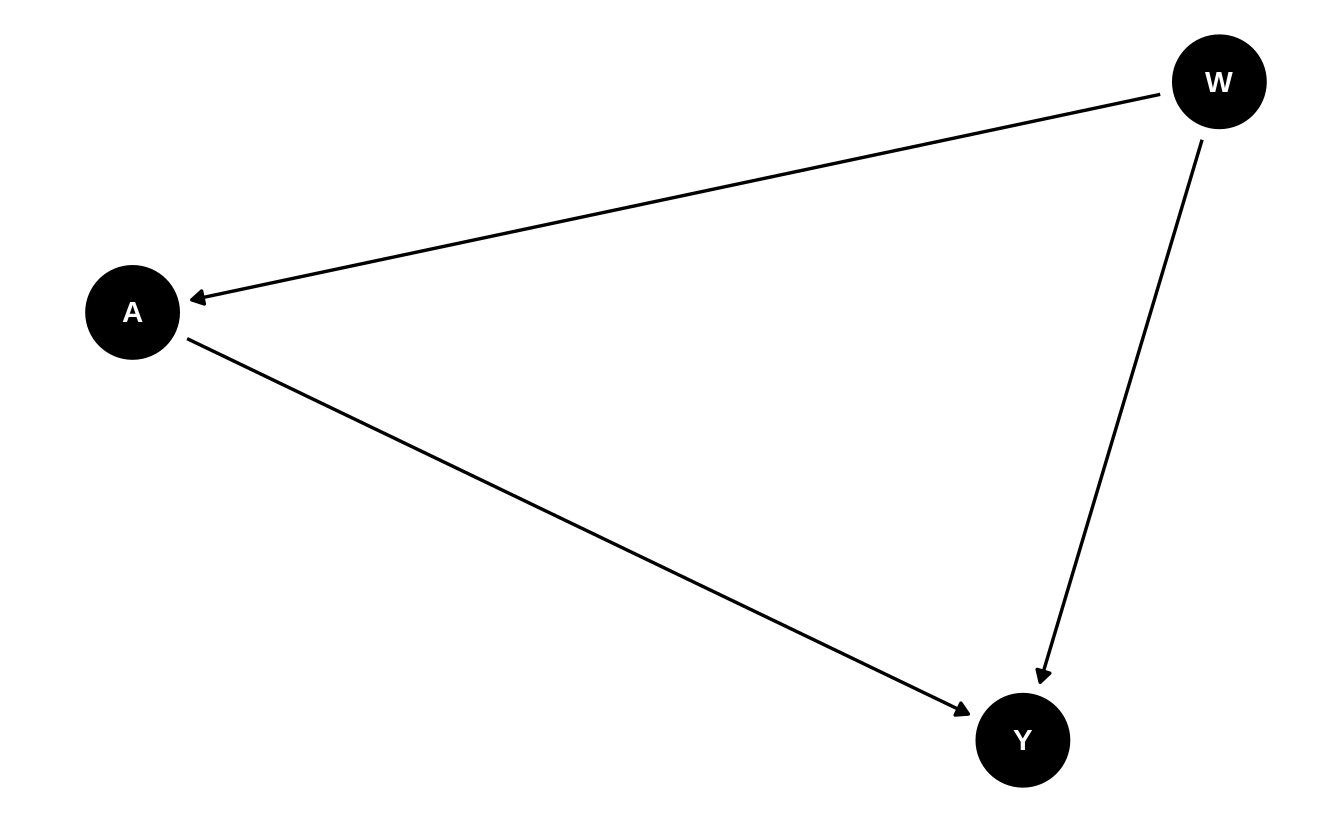
\includegraphics[width=0.8\linewidth]{02-roadmap_files/figure-latex/simple-DAG-1} \end{center}

While directed acyclic graphs (DAGs) like above provide a convenient means by
which to visualize causal relations between variables, the same causal relations
among variables can be represented via a set of structural equations, which
define the non-parametric structural equation model (NPSEM):
\begin{align*}
  W &= f_W(U_W) \\
  A &= f_A(W, U_A) \\
  Y &= f_Y(W, A, U_Y),
\end{align*}
where \(U_W\), \(U_A\), and \(U_Y\) represent the unmeasured exogenous background
characteristics that influence the value of each variable. In the NPSEM, \(f_W\),
\(f_A\) and \(f_Y\) denote that each variable (for \(W\), \(A\) and \(Y\), respectively)
is a function of its parents and unmeasured background characteristics, but note
that there is no imposition of any particular functional constraints(e.g.,
linear, logit-linear, only one interaction, etc.). For this reason, they are
called non-parametric structural equation models (NPSEMs). The DAG and set of
nonparametric structural equations represent exactly the same information and so
may be used interchangeably.

The first hypothetical experiment we will consider is assigning exposure to the
whole population and observing the outcome, and then assigning no exposure to
the whole population and observing the outcome. On the nonparametric structural
equations, this corresponds to a comparison of the outcome distribution in the
population under two interventions:

\begin{enumerate}
\def\labelenumi{\arabic{enumi}.}
\tightlist
\item
  \(A\) is set to \(1\) for all individuals, and
\item
  \(A\) is set to \(0\) for all individuals.
\end{enumerate}

These interventions imply two new nonparametric structural equation models. For
the case \(A = 1\), we have
\begin{align*}
  W &= f_W(U_W) \\
  A &= 1 \\
  Y(1) &= f_Y(W, 1, U_Y),
\end{align*}
and for the case \(A=0\),
\begin{align*}
  W &= f_W(U_W) \\
  A &= 0 \\
  Y(0) &= f_Y(W, 0, U_Y).
\end{align*}

In these equations, \(A\) is no longer a function of \(W\) because we have
intervened on the system, setting \(A\) deterministically to either of the values
\(1\) or \(0\). The new symbols \(Y(1)\) and \(Y(0)\) indicate the outcome variable in
our population if it were generated by the respective NPSEMs above; these are
often called \emph{counterfactuals} (since they run contrary-to-fact). The difference
between the means of the outcome under these two interventions defines a
parameter that is often called the ``average treatment effect'' (ATE), denoted
\begin{equation}\label{eqn:ate}
  ATE = \mathbb{E}_X(Y(1)-Y(0)),
\end{equation}
where \(\mathbb{E}_X\) is the mean under the theoretical (unobserved) full data
\(X = (W, Y(1), Y(0))\).

Note, we can define much more complicated interventions on NPSEM's, such as
interventions based upon rules (themselves based upon covariates), stochastic
rules, etc. and each results in a different targeted parameter and entails
different identifiability assumptions discussed below.

\hypertarget{identifiability}{%
\subsection*{Identifiability}\label{identifiability}}


Because we can never observe both \(Y(0)\) (the counterfactual outcome when \(A=0\))
and \(Y(1)\) (similarly, the counterfactual outcome when \(A=1\)), we cannot
estimate \ref{eqn:ate} directly. Instead, we have to make assumptions under
which this quantity may be estimated from the observed data \(O \sim P_0\) under
the data-generating distribution \(P_0\). Fortunately, given the causal model
specified in the NPSEM above, we can, with a handful of untestable assumptions,
estimate the ATE, even from observational data. These assumptions may be
summarized as follows.

\begin{enumerate}
\def\labelenumi{\arabic{enumi}.}
\tightlist
\item
  The causal graph implies \(Y(a) \perp A\) for all \(a \in \mathcal{A}\), which
  is the \emph{randomization} assumption. In the case of observational data, the
  analogous assumption is \emph{strong ignorability} or \emph{no unmeasured confounding}
  \(Y(a) \perp A \mid W\) for all \(a \in \mathcal{A}\);
\item
  Although not represented in the causal graph, also required is the assumption
  of no interference between units, that is, the outcome for unit \(i\) \(Y_i\) is
  not affected by exposure for unit \(j\) \(A_j\) unless \(i=j\);
\item
  \emph{Consistency} of the treatment mechanism is also required, i.e., the outcome
  for unit \(i\) is \(Y_i(a)\) whenever \(A_i = a\), an assumption also known as ``no
  other versions of treatment'';
\item
  It is also necessary that all observed units, across strata defined by \(W\),
  have a bounded (non-deterministic) probability of receiving treatment --
  that is, \(0 < \mathbb{P}(A = a \mid W) < 1\) for all \(a\) and \(W\)). This assumption
  is referred to as \emph{positivity} or \emph{overlap}.
\end{enumerate}

\emph{Remark}: Together, (2) and (3), the assumptions of no interference and
consistency, respectively, are jointly referred to as the \emph{stable unit
treatment value assumption} (SUTVA).

Given these assumptions, the ATE may be re-written as a function of \(P_0\),
specifically
\begin{equation}\label{eqn:estimand}
  ATE = \mathbb{E}_0(Y(1) - Y(0)) = \mathbb{E}_0
    \left(\mathbb{E}_0[Y \mid A = 1, W] - \mathbb{E}_0[Y \mid A = 0, W]\right).
\end{equation}
In words, the ATE is the difference in the predicted outcome values for each subject, under the
contrast of treatment conditions (\(A = 0\) vs.~\(A = 1\)), in the population,
averaged over all observations. Thus, a parameter of a theoretical ``full'' data
distribution can be represented as an estimand of the observed data
distribution. Significantly, there is nothing about the representation in
\ref{eqn:estimand} that requires parameteric assumptions; thus, the regressions
on the right hand side may be estimated freely with machine learning. With
different parameters, there will be potentially different identifiability
assumptions and the resulting estimands can be functions of different components
of \(P_0\). We discuss several more complex estimands in later sections of this
handbook.

\hypertarget{natural}{%
\chapter{The Natural Direct and Indirect Effects}\label{natural}}

{[}TO FILL IN{]}

\hypertarget{interventional}{%
\chapter{The Interventional Direct and Indirect Effects}\label{interventional}}

{[}TO FILL IN{]}

\hypertarget{stochastic}{%
\chapter{The Stochastic Direct and Indirect Effects}\label{stochastic}}

{[}TO FILL IN{]}

  \bibliography{book.bib,packages.bib}

\backmatter
\printindex

\end{document}
